\documentclass[20pt]{article}

\usepackage[english]{babel}
\usepackage[utf8x]{inputenc}
% \usepackage{amsmath}
\usepackage{graphicx}
\usepackage[margin=0.8in]{geometry}

\title{AS205:Ocean Dynamics(Assignment 2)}
\author{Parag Shende}

\begin{document}
\maketitle
\hrule

\section*{Introduction}

We describe the seasonal means of sea surface temperature(SST) and sea surface salinity(SSS) in the Bay of Bengal and Arabian Sea. 
This is undertaken to study the spatial and temporal patterns of the two fields. The seasonal means are constructed for the year 2022.

\section*{Datasets}

The datasets used in this analysis is as follows:

\begin{itemize}
    \item \textbf{Sea Surface Temperature(SST)} : GHRSST data.
    \item \textbf{Sea Surface Salinity(SSS)} : SMAP data.
\end{itemize}

\section*{Methodology}

The datasets are choosen for the domain of $40^{\circ} E$ to $100^{\circ}E$ and $0^{\circ} N$ to $25^{\circ} N$. This covers the
North Indian ocean. We then calculate the seasonal mean with the following seasons:
\begin{itemize}
    \item \textbf{Spring} : January, February, March, April
    \item \textbf{Summer} : May, June, July, August
    \item \textbf{Winter} : September, October, November, December
\end{itemize}

We contrast the differences in spatial and temporal features in the SST and SSS fields for the 
Arabian Sea and Bay of Bengal. 

\section*{Sea Surface Temperature}

\subsection*{Spring}

\begin{figure}
    \centering
    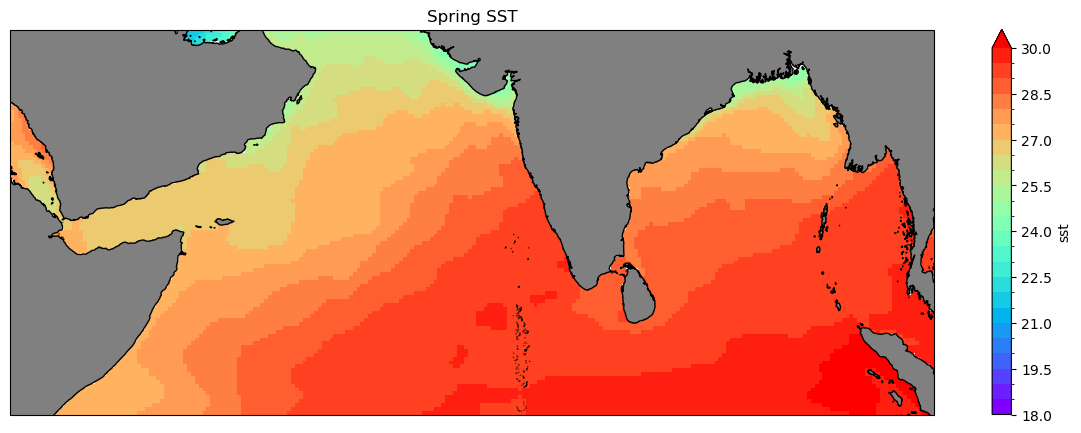
\includegraphics[width=0.7\textwidth]{spring_sst.png}
    \caption{SST seasonal mean for spring}
\end{figure}

\begin{itemize}
    \item The seasonal mean for spring is plotted in Figure 1. 
    \item The Equatorial Indian ocean is considerably warmer than the Northern Indian ocean.
    \item The freshwater forcing in Bay of Bengal near the head bay and the Northern part of Eastern Arabian sea lead to cooler SST.
    \item The Arabian Sea is cooler than the Bay of Bengal on an average. This might be due to strong stratification in the Bay of Bengal which leads to warmer SST.
\end{itemize}

\subsection*{Summer}

\begin{figure}
    \centering
    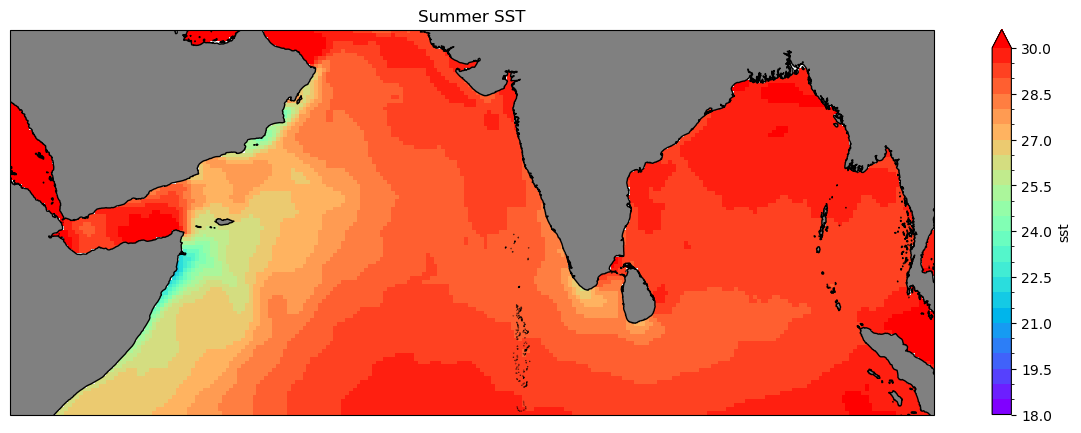
\includegraphics[width=0.7\textwidth]{summer_sst.png}
    \caption{SST seasonal mean for summer}
\end{figure}

\begin{itemize}
    \item Comparing it with spring by summer, we see considerable warming in Northern Indian ocean in all the basins.
    \item Though the equatorial Indian ocean seems to have the same SSTs.
    \item The eastern coast off Somali and Saudi Arabia seems to have lower SSTs compared with spring that could be due to upwelling happening there.
    \item The northern Bay of Bengal is warmer as compared to southern bay due to strong stratification present.
\end{itemize}

\subsection*{Winter}

\begin{figure}
    \centering
    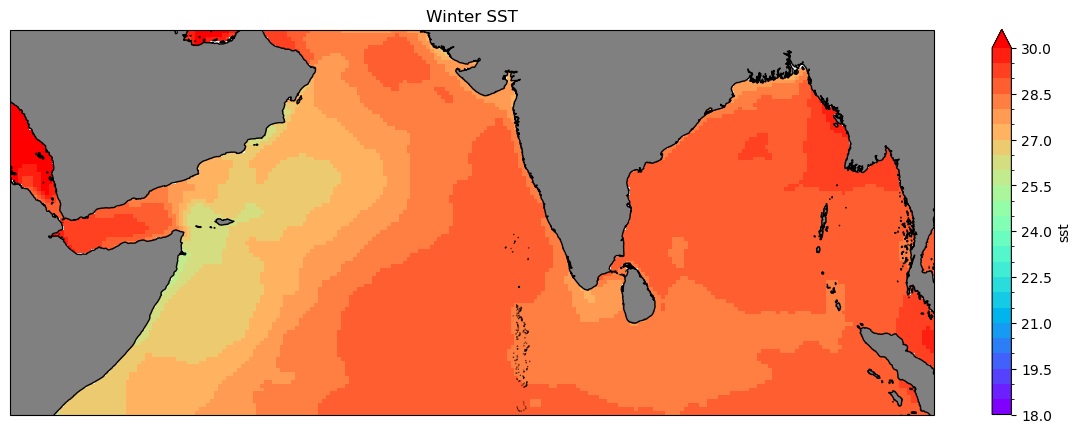
\includegraphics[width=0.7\textwidth]{winter_sst.png}
    \caption{SST seasonal mean for winter}
\end{figure}

\begin{itemize}
    \item As expected, the coolest SSTs are observed in winter. This is shown in Figure 3.
    \item On an average, again the Arabian sea is cooler than the Bay of Bengal.
\end{itemize}


\section*{Sea Surface Salinity}

\subsection*{Spring}

\begin{figure}
    \centering
    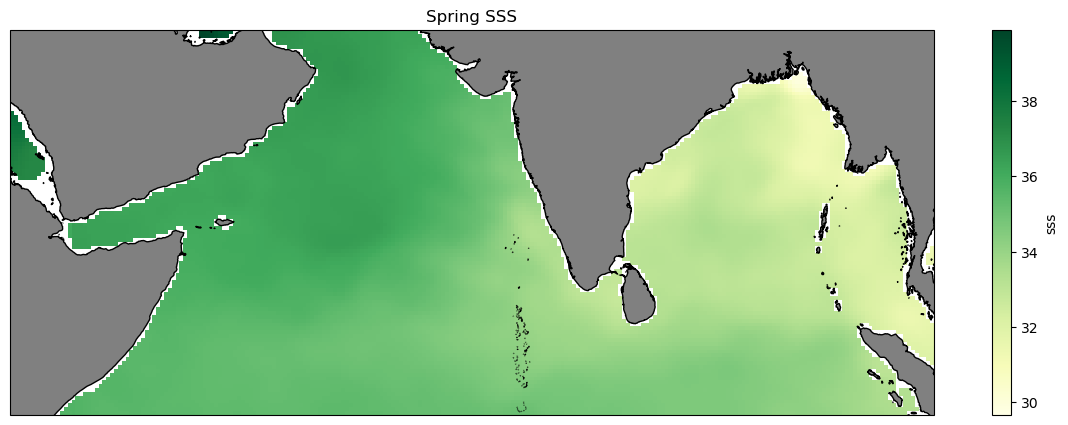
\includegraphics[width=0.7\textwidth]{spring_sss.png}
    \caption{SSS seasonal mean for spring}
\end{figure}

\begin{itemize}
    \item The Bay of Bengal is fresher as compared to Arabian sea due to large freshwater forcing.
    \item The Arabian sea has drainage from Gulf of Aden and Red Sea which are salty water bodies.
\end{itemize}

\subsection*{Summer}

\begin{figure}
    \centering
    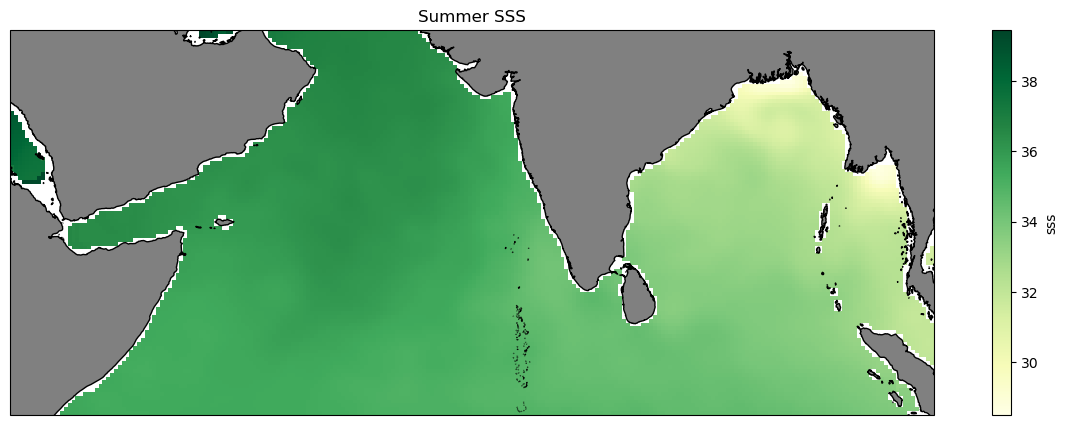
\includegraphics[width=0.7\textwidth]{summer_sss.png}
    \caption{SSS seasonal mean for summer}
\end{figure}

\begin{itemize}
    \item By summer, the Arabian sea has become saltier due to evaporation.
    \item The Bay of Bengal also shows mild saltening.
\end{itemize}

\subsection*{Winter}

\begin{figure}
    \centering
    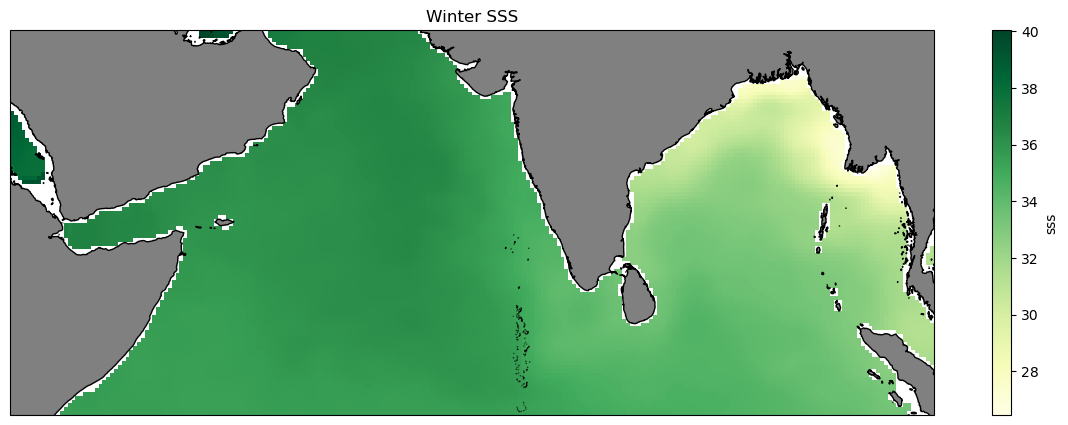
\includegraphics[width=0.7\textwidth]{winter_sss.png}
    \caption{SSS seasonal mean for winter}
\end{figure}

\begin{itemize}
    \item The Arabian sea continues to get saltier and the southern Arabian sea is also saltier as compared to spring and summer.
    \item The river water discharge in the northern Bay leads to reduction in salinity and this is clearly seen in the Figure 6.
    \item Hence, the northern bay is fresher in winter as compared to summer or spring.
\end{itemize}

\section*{Conclusions}

\begin{itemize}
    \item We compared the seasonal means of SST and SSS for northern Indian ocean.
    \item On an average the Arabian sea is saltier than the Bay of Bengal. This is primarly due to large freshwater influx in the bay.
    \item The Arabian sea is cooler than the Bay of Bengal as strong stratification in the bay prevents the deepening of mixed layer and hence the shortwave heat is surface trapped.
\end{itemize}

\end{document}